% chapters/03-success-stories.tex

\chapter{Success Stories and Lessons Learned}

\begin{importantbox}
This chapter presents composite case studies based on real success patterns in the Nigerian market. Each story highlights key success factors, challenges overcome, and practical lessons learned.
\end{importantbox}

\section{United Kingdom: FinTech Scale-up Story}

\subsection{Meet Sarah: Ex-Investment Banker Turned FinTech Founder}
\begin{tcolorbox}[colback=white,colframe=primarydark,title=\textbf{Entrepreneur Profile}]
\begin{itemize}
    \item \textbf{Background:} 15 years in investment banking
    \item \textbf{Age:} 45
    \item \textbf{Previous Experience:} Global financial services
    \item \textbf{Target Market:} Cross-border payments
\end{itemize}
\end{tcolorbox}

\subsection{The Journey}
Sarah's path to success in Nigeria's fintech space...

\begin{figure}[h]
    \centering
    
\begin{tikzpicture}
        % Journey timeline
        \draw[thick,->] (0,0) -- (12,0);
        \foreach \x/\label in {0/Market Research,3/Initial Entry,6/Product Launch,9/Scale-up,12/Expansion}
        {
            \draw (\x,0.2) -- (\x,-0.2);
            \node[rotate=45, anchor=west] at (\x,-0.3) {\label};
        }
    \end{tikzpicture}
    \caption{Sarah's Market Entry Timeline}
\end{figure}

\subsection{Key Success Factors}
\begin{itemize}
    \item Regulatory compliance strategy
    \item Local partnership development
    \item Market adaptation approach
\end{itemize}

\subsection{Challenges Overcome}
\begin{center}
\begin{tabular}{p{0.4\textwidth}|p{0.5\textwidth}}
    \textbf{Challenge} & \textbf{Solution Applied} \\
    \hline
    Regulatory complexity & Strategic local partnerships \\
    Market skepticism & Phased rollout approach \\
    Technical integration & Hybrid technology stack \\
\end{tabular}
\end{center}

\section{United States: E-commerce Platform Launch}

\subsection{Meet Mike: Tech Entrepreneur}
\begin{tcolorbox}[colback=white,colframe=primarydark,title=\textbf{Entrepreneur Profile}]
\begin{itemize}
    \item \textbf{Background:} Serial tech entrepreneur
    \item \textbf{Age:} 35
    \item \textbf{Previous Experience:} B2B SaaS platforms
    \item \textbf{Target Market:} Digital commerce
\end{itemize}
\end{tcolorbox}

\subsection{Market Adaptation Strategy}
\begin{figure}[h]
    \centering
    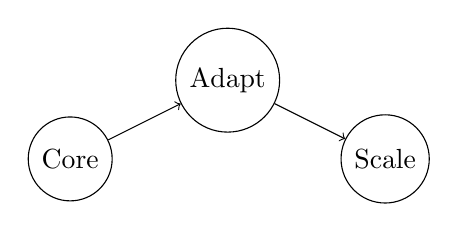
\begin{tikzpicture}
        % Strategy visualization
        \node[draw,circle] (core) at (0,0) {Core};
        \node[draw,circle] (adapt) at (2,1) {Adapt};
        \node[draw,circle] (scale) at (4,0) {Scale};
        \draw[->] (core) -- (adapt);
        \draw[->] (adapt) -- (scale);
    \end{tikzpicture}
    \caption{Market Adaptation Framework}
\end{figure}

\section{UAE: Trade Company Establishment}

\subsection{Meet Ahmed: Trade Specialist}
\begin{tcolorbox}[colback=white,colframe=primarydark,title=\textbf{Entrepreneur Profile}]
\begin{itemize}
    \item \textbf{Background:} International trade expert
    \item \textbf{Age:} 50
    \item \textbf{Previous Experience:} Global supply chain
    \item \textbf{Target Market:} Import/Export
\end{itemize}
\end{tcolorbox}

\subsection{Market Penetration Approach}
\begin{figure}[h]
    \centering
    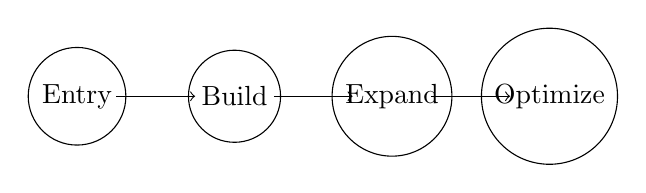
\begin{tikzpicture}
        % Market penetration stages
        \foreach \x/\y/\label in {0/0/Entry,2/0/Build,4/0/Expand,6/0/Optimize}
        {
            \node[draw,circle] at (\x,\y) {\label};
            \ifnum\x<6
                \draw[->] (\x+0.5,\y) -- (\x+1.5,\y);
            \fi
        }
    \end{tikzpicture}
    \caption{Market Penetration Stages}
\end{figure}

\section{Canadian: AgriTech Innovation}

\subsection{Meet Lisa: AgriTech Innovator}
\begin{tcolorbox}[colback=white,colframe=primarydark,title=\textbf{Entrepreneur Profile}]
\begin{itemize}
    \item \textbf{Background:} Agricultural technology
    \item \textbf{Age:} 40
    \item \textbf{Previous Experience:} Sustainable farming
    \item \textbf{Target Market:} Farm automation
\end{itemize}
\end{tcolorbox}

\subsection{Partnership Development}
\begin{center}
\begin{tabular}{p{0.3\textwidth}|p{0.3\textwidth}|p{0.3\textwidth}}
    \textbf{Partner Type} & \textbf{Role} & \textbf{Impact} \\
    \hline
    Local Farms & Testing & Market validation \\
    Tech Partners & Integration & Solution scaling \\
    Government & Support & Market access \\
\end{tabular}
\end{center}

\begin{communitybox}
Access extended case studies and entrepreneur interviews on the Africa Growth Circle:
\begin{itemize}
    \item Detailed video interviews
    \item Monthly success story updates
    \item Live Q\&A sessions with featured entrepreneurs
    \item Industry-specific case studies
\end{itemize}
Visit circle.counseal.com for more success stories.
\end{communitybox}

% End of chapter workshop
\begin{workshopbox}
\textbf{Chapter 3 Learning Application Workshop}

1. Success Pattern Analysis
\begin{itemize}
    \item Key success factors identified: \_\_\_\_\_\_\_\_\_
    \item Relevant factors for your business: \_\_\_\_\_\_\_\_\_
    \item Implementation strategy: \_\_\_\_\_\_\_\_\_
\end{itemize}

2. Challenge Mitigation Planning
\begin{itemize}
    \item Anticipated challenges: \_\_\_\_\_\_\_\_\_
    \item Proposed solutions: \_\_\_\_\_\_\_\_\_
    \item Resource requirements: \_\_\_\_\_\_\_\_\_
\end{itemize}

3. Partnership Strategy
\begin{itemize}
    \item Target partners: \_\_\_\_\_\_\_\_\_
    \item Partnership objectives: \_\_\_\_\_\_\_\_\_
    \item Engagement approach: \_\_\_\_\_\_\_\_\_
\end{itemize}

Access additional case studies and success stories on the Africa Growth Circle platform.
\end{workshopbox}

\begin{importantbox}
In Chapter 4, we'll translate these success patterns into a practical 90-day action plan for your market entry.
\end{importantbox}